\section{Experimental Evaluation} \label{sec:experiment}

We experimentally evaluated \nn{}, showing its ability to run with an adaptive minimum threshold that mitigate non-termination and improve energy efficiency. 
\nn{}'s runtime energy profiling presents a low and relatively consistent error across different task scales. 
We show that, despite with reduced capacitance, \nn{} is able to adapt \nm{V}{th} to meet a target end voltage \nm{V}{end} until the highest threshold is reached, while the fixed-threshold comparison \debs{} fails.
We also show that \nn{} improves performance over \debs{} and Samoyed with a PV panel supply owning to its reduced operating voltage. 

\subsection{Experimental Setup and Benchmarks}

A PV panel (Sanyo AM-1417CA) provided the sole power supply for the system. 
It is covered in a black box with a white LED light as the only energy source, producing a consistent supply characteristic (as shown in \fref{fig:pv_iv}) during the experiments.
For the experiment on capacitance reduction only, we instead use a constant low-current supply so as to examine whether the system is able to survive with little energy income during task execution. 

Three common peripheral tasks in IoT sensors were used as the benchmarks for evaluation. 
\begin{itemize}
    \item \textbf{DMA}: Data transfer using an on-chip DMA module, frequently used in data logging.
    \item \textbf{AES}: AES encryption using an on-chip AES accelerator processing up to 4KB data at a time for secure communication.
    \item \textbf{RF}:  Wireless communication through an external nRF24L01 radio module, transmitting a payload up to 96B at a time, configured as a 2Mbps air data rate and a \SI{0}{\decibel{m}} output power. 
    The radio module is connected through an LDO with a \SI{2}{\volt} output voltage to lower the quiescent current consumption, with a \SI{10}{\micro\farad} at the LDO's low side. 
\end{itemize}

% No state retention
% Comparisons: DEBS, Samoyed (without scaling), Plain C (for evaluating overheads)
% Samoyed scales down the atomic task if it fails to complete (but never scales back). 
% It uses an "energy profiler" in previous work to test the whether the smallest scale of all peripheral tasks and randomised inputs can successfully complete. 
% They suggested it is appropriate to set an energy capacity that can run the smallest scale of an operation for hundreds of times in one active cycle. 
% Hence, it does not look for a threshold for a task with a specific configuration, but instead its aim is to minimise the chance of non-termination in practice by giving a high margin.

\subsection{Profiling Accuracy}
% Question: How does our profiling approach perform in terms of accuracy?
% Accuracy compared to manual measurement.

\begin{figure}[t]
    \centering
    \begin{tikzpicture}
    \begin{groupplot}[
        group style={group size=3 by 1,horizontal sep=5pt},
        width=0.4\columnwidth, height=5cm,
        xmin=-13,xmax=13,
        ymin=0,ymax=110,
        xtick distance=5,
        ytick distance=20,
        xticklabel pos=bottom,
        every tick label/.append style={font=\small},
        minor x tick num=0,
        area style,
        xlabel={Error (\SI{}{\milli\volt})},
        xlabel style={yshift=3pt,},
        title style={at={(0.5,0)},anchor=north,yshift=-1.5cm},
        ]

        \nextgroupplot [title={(a) DMA},yticklabel={\pgfmathprintnumber\tick\%}]
        \addplot 
            plot [ybar interval,mark=no,black,fill=Set1-B,]
            table [x=v_error,y=repa_dma,col sep=comma] {ch5_optic/figures/profiling_accuracy/profiling_accuracy.csv};
        \node (n1) at (axis cs:0,100) {};
        \node (n2) at (axis cs:0,0) {};
        \draw [color=Set1-A,ultra thick,dashed] (n2) -- (n1);
        \node [anchor=north, font=\footnotesize, color=Set1-A] at (axis cs:0,108) {$\Delta V_{\text{task}}$=\SI{107}{\milli\volt}};

        \nextgroupplot [title={(b) AES},yticklabel=\empty]
        \addplot 
            plot [ybar interval,mark=no,black,fill=Set1-B,]
            table [x=v_error,y=repa_aes,col sep=comma] {ch5_optic/figures/profiling_accuracy/profiling_accuracy.csv};
        \node (n1) at (axis cs:0,100) {};
        \node (n2) at (axis cs:0,0) {};
        \draw [color=Set1-A,ultra thick,dashed] (n2) -- (n1);
        \node [anchor=north, font=\footnotesize, color=Set1-A] at (axis cs:0,108) {$\Delta V_{\text{task}}$=\SI{583}{\milli\volt}};

        \nextgroupplot [title={(c) RF},yticklabel=\empty]
        \addplot 
            plot [ybar interval,mark=no,black,fill=Set1-B,]
            table [x=v_error,y=repa_radio,col sep=comma] {ch5_optic/figures/profiling_accuracy/profiling_accuracy.csv};
        \node (n1) at (axis cs:0,100) {};
        \node (n2) at (axis cs:0,0) {};
        \draw [color=Set1-A,ultra thick,dashed] (n2) -- (n1);
        \node [anchor=north, font=\footnotesize, color=Set1-A] at (axis cs:0,108) {$\Delta V_{\text{task}}$=\SI{720}{\milli\volt}};
    \end{groupplot}
    \end{tikzpicture}
    \caption{\nn{} Profiling accuracy. }
    \label{fig:profiling_accuracy}
\end{figure} 

% Old figure
% \begin{figure*}[t]
%     \centering
%     \begin{tikzpicture}
%     \begin{groupplot}[
%         group style={group size=3 by 2, vertical sep=43pt},
%         width=0.7\columnwidth, height=3.7cm,
%         xmin=-15,xmax=15,
%         ymin=0,ymax=100,
%         xtick distance=5,
%         % xtick pos=top,
%         xticklabel pos=bottom,
%         yticklabel={\pgfmathprintnumber\tick\%},
%         every tick label/.append style={font=\small},
%         minor x tick num=0,
%         area style,
%         xlabel={Error (\SI{}{\milli\volt})},
%         xlabel style={yshift=3pt,},
%         title style={yshift=-7pt,},
%         ]

%         \nextgroupplot [title={(a) REPA, DMA Transfer}]
%         \addplot 
%             plot [ybar interval,mark=no,black,fill=Set1-B,]
%             table [x=v_error,y=repa_dma,col sep=comma] {figures/profiling_accuracy/profiling_accuracy.csv};
%         \node [anchor=north, font=\footnotesize, color=Set1-A] (n1) at (axis cs:0,100) {\SI{107}{\milli\volt}};
%         \node (n2) at (axis cs:0,0) {};
%         \draw [color=Set1-A,thick,dashed] (n2) -- (n1);

%         \nextgroupplot [title={(b) REPA, AES Encryption}]
%         \addplot 
%             plot [ybar interval,mark=no,black,fill=Set1-B,]
%             table [x=v_error,y=repa_aes,col sep=comma] {figures/profiling_accuracy/profiling_accuracy.csv};
%         \node [anchor=north, font=\footnotesize, color=Set1-A] (n1) at (axis cs:0,100) {\SI{583}{\milli\volt}};
%         \node (n2) at (axis cs:0,0) {};
%         \draw [color=Set1-A,thick,dashed] (n2) -- (n1);

%         \nextgroupplot [title={(c) REPA, Radio Transmission}]
%         \addplot 
%             plot [ybar interval,mark=no,black,fill=Set1-B,]
%             table [x=v_error,y=repa_radio,col sep=comma] {figures/profiling_accuracy/profiling_accuracy.csv};
%         \node [anchor=north, font=\footnotesize, color=Set1-A] (n1) at (axis cs:0,100) {\SI{720}{\milli\volt}};
%         \node (n2) at (axis cs:0,0) {};
%         \draw [color=Set1-A,thick,dashed] (n2) -- (n1);

%         \nextgroupplot [title={(d) Naive, DMA Transfer}]
%         \addplot 
%             plot [ybar interval,mark=no,black,fill=Set1-B,]
%             table [x=v_error,y=naive_dma,col sep=comma] {figures/profiling_accuracy/profiling_accuracy.csv};
%         \node [anchor=north, font=\footnotesize, color=Set1-A] (n1) at (axis cs:0,100) {\SI{107}{\milli\volt}};
%         \node (n2) at (axis cs:0,0) {};
%         \draw [color=Set1-A,thick,dashed] (n2) -- (n1);

%         \nextgroupplot [title={(e) Naive, AES Encryption}]
%         \addplot 
%             plot [ybar interval,mark=no,black,fill=Set1-B,]
%             table [x=v_error,y=naive_aes,col sep=comma] {figures/profiling_accuracy/profiling_accuracy.csv};
%         \node [anchor=north, font=\footnotesize, color=Set1-A] (n1) at (axis cs:0,100) {\SI{583}{\milli\volt}};
%         \node (n2) at (axis cs:0,0) {};
%         \draw [color=Set1-A,thick,dashed] (n2) -- (n1);

%         \nextgroupplot [title={(f) Naive, Radio Transmission}]
%         \addplot 
%             plot [ybar interval,mark=no,black,fill=Set1-B,]
%             table [x=v_error,y=naive_radio,col sep=comma] {figures/profiling_accuracy/profiling_accuracy.csv};
%         \node [anchor=north, font=\footnotesize, color=Set1-A] (n1) at (axis cs:0,100) {\SI{720}{\milli\volt}};
%         \node (n2) at (axis cs:0,0) {};
%         \draw [color=Set1-A,thick,dashed] (n2) -- (n1);
        
%     \end{groupplot}


%     \end{tikzpicture}
%     \caption{Profiling accuracy. }
%     \label{fig:profiling_accuracy}
% \end{figure*} 


We first measured the profiling accuracy of \nn{}'s runtime energy profiling ability. 
A hundred profiling results were obtained for each workload. 
Manual profiling was also conducted by disconnecting the power supply during task execution and reading $\Delta\nmm{V}{task}$ from a scope, and used as a reference that we evaluate the profiling results against. 
The results are divided in a \SI{5}{\milli\volt} step because the resolution of our scope is \SI{5}{\milli\volt}, below which the manual profiled reference is not even accurate. 

As shown in \fref{fig:profiling_accuracy}, the profiling errors are low and relatively consistent (mostly within \SI{5}{\milli\volt}) across the three workload with different levels of energy consumption. 
The error becomes insignificant with energy-hungry tasks, e.g. RF. 
Compared to the step of voltage thresholds in our implementation (around \SI{30}{\milli\volt}), this \SI{5}{\milli\volt} error is acceptable as it can convert to a relatively stable threshold assuming a fixed energy consumption. 

Additionally, the average profiling results are shown to be a slightly higher than the reference, which 
seems to contradict the theoretical error that is supposed to make the profiling undershoot.
This is majorly due to a positive error in the MCU's internal 1/2 \nm{V}{cc} divider from an observation that the Naive approach produced a higher reading. 
This also evidences that the theoretical error is insignificant and easily compensated by other factors. 


\subsection{Reliability with Dynamic Energy Consumption}

We evaluated whether \nn{} can adapt to variability in IPSs and keep making forward progress.
We classified the variability in three categories according to the frequency of these changes: 
\begin{itemize}
    \item \textbf{Changing once}, such as new workloads, devices, and components.
    \item \textbf{Changing infrequently}, such as capacitor ageing, device ageing, temperature changes, and configurations that last for a long term.
    \item \textbf{Changing frequently}, such as variable data sizes and peripheral configurations that can frequently change. 
\end{itemize}
To reduce similar results, we show one example in each category to illustrate \nn{}'s adaptation to variability. 

\subsubsection{Changing once}
% new operations, device, components

\begin{figure}
    \centering
    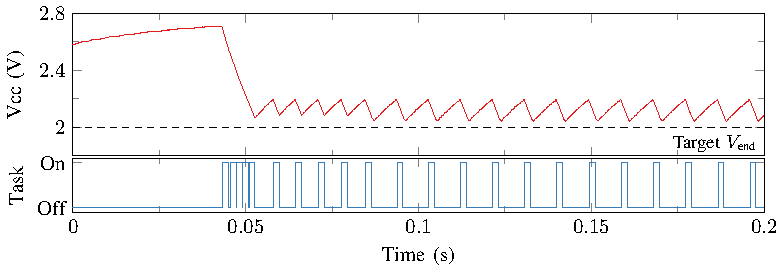
\includegraphics[width=\columnwidth]{ch5_optic/figures/v_trace/v_trace.pdf}
    \caption{A voltage trace of \nn{} adapting to a new operation on a new device. }
    \label{fig:v_trace}
\end{figure}

\fref{fig:v_trace} shows an example of how \nn{} adapts its threshold to a new workload and a new device. 
The system runs an AES-128 encryption on 1KB data repetitively . 
The algorithm does not have any knowledge on the energy consumption of the platform or the workload.
The system first waits for the initial profiling threshold, which is set at \SI{2.7}{\volt} in this case. 
Then it performs energy profiling as this is the first time it executes this task. 
The next threshold for the task is then adapted to a lower one.
In the following execution, the system is able to maintain the same threshold that guarantees the completion of the task. 
The end voltage after completing a task matches closely with the target \nm{V}{end}, with a small margin that comes from both the round-up threshold and the energy harvested during the task execution. 
The above example shows \nn{}'s ability to adapt to a new workload or device, obviating the need for manual energy profiling for various scenarios, e.g. updating workloads or deploying new devices. 

\subsubsection{Changing infrequently}
% Variability in capacitance due to ageing / tolerance (slowly changing)
% Actually the mechanism isn't any different from changing once. 


% \begin{figure*}[t]
%     \centering
%     \begin{tikzpicture}
%     \begin{groupplot}[
%         group style={group size=1 by 2,vertical sep=2pt},
%         width=0.5\columnwidth,
%         xmin=0,xmax=80,
%         every tick label/.append style={font=\small},
%         minor x tick num=0,
%         ]

%         % (a) upper
%         \nextgroupplot[
%             const plot,
%             height=4cm,
%             ymin=-0.2,ymax=1.2,
%             ytick distance=1,
%             xticklabel=\empty,
%             yticklabels={,Fail,Done},
%             legend style={
%                 anchor=west,
%                 at={(0.02,0.5)},
%                 font=\footnotesize,
%                 legend columns=2,
%             },
%             ]
%         \addplot 
%             plot [Set1-B,mark=o]
%             table [x=cap_reduction,y=opta_perf,col sep=comma] {ch5_optic/figures/capacitance/cap_test_dma.csv};
%         \addplot 
%             plot [Set1-A,mark=square]
%             table [x=cap_reduction,y=debs_perf,col sep=comma] {ch5_optic/figures/capacitance/cap_test_dma.csv};
%         \legend{\nn{},\debs{}}

%         % (b) upper
%         \nextgroupplot[
%             const plot,
%             height=4cm,
%             ymin=-0.2,ymax=1.2,
%             ytick distance=1,
%             xticklabel=\empty,
%             yticklabels={,Fail,Done},
%             legend style={
%                 anchor=west,
%                 at={(0,0.5)},
%                 font=\footnotesize,
%                 legend columns=2,
%             },
%             ]
%         \addplot 
%             plot [Set1-B,mark=o]
%             table [x=cap_reduction,y=opta_perf,col sep=comma] {ch5_optic/figures/capacitance/cap_test_aes.csv};
%         \addplot 
%             plot [Set1-A,mark=square]
%             table [x=cap_reduction,y=debs_perf,col sep=comma] {ch5_optic/figures/capacitance/cap_test_aes.csv};
%         % \legend{\nn{},\debs{}}

%         % (a) lower
%         \nextgroupplot[
%             height=6cm,
%             title={(a) DMA},
%             title style={at={(0.5,0)},anchor=north,yshift=-30pt,},
%             ymin=1.7,ymax=2.5,
%             xlabel={Capacitance Reduction},
%             ylabel={Start \& End Voltage (V)},
%             ytick distance=0.2,
%             xlabel style={yshift=3pt,},
%             xticklabel={\pgfmathprintnumber\tick\%},
%             legend style={
%                 anchor=north west,
%                 at={(0.02,0.98)},
%                 font=\footnotesize,
%                 legend columns=2,
%             },
%             ]
%         \addplot 
%             plot [Set1-B,mark=*]
%             table [x=cap_reduction,y=opta_v_start,col sep=comma] {ch5_optic/figures/capacitance/cap_test_dma.csv};
%         \addplot 
%             plot [Set1-B,mark=o]
%             table [x=cap_reduction,y=opta_v_end,col sep=comma] {ch5_optic/figures/capacitance/cap_test_dma.csv};
%         \addplot 
%             plot [Set1-A,mark=square*]
%             table [x=cap_reduction,y=debs_v_start,col sep=comma] {ch5_optic/figures/capacitance/cap_test_dma.csv};
%         \addplot 
%             plot [Set1-A,mark=square]
%             table [x=cap_reduction,y=debs_v_end,col sep=comma] {ch5_optic/figures/capacitance/cap_test_dma.csv};
%         \draw [thick,dashed] (axis cs:0,2) -- (axis cs:80,2);
%         \node [anchor=north east,font=\small] at (axis cs:80,2) {Target $V_{\text{end}}$};
%         \draw [thick,dashed] (axis cs:0,1.8) -- (axis cs:80,1.8);
%         \node [anchor=north east,font=\small] at (axis cs:80,1.8) {Fail};
%         \legend{\ ,\nn{} $V_{\text{start}}\ V_{\text{end}}$,\ ,\debs{} $V_{\text{start}}\ V_{\text{end}}$}

%         % (b) lower
%         \nextgroupplot[
%             height=6cm,
%             title={(b) AES},
%             title style={at={(0.5,0)},anchor=north,yshift=-30pt,},
%             ymin=1.55,ymax=3.7,
%             xlabel={Capacitance Reduction},
%             ytick distance=0.5,
%             extra y ticks={1.8},
%             xlabel style={yshift=3pt,},
%             xticklabel={\pgfmathprintnumber\tick\%},
%             legend style={
%                 anchor=north west,
%                 at={(0,1)},
%                 font=\footnotesize,
%                 legend columns=2,
%             },
%             ]
%         \addplot 
%             plot [Set1-B,mark=*]
%             table [x=cap_reduction,y=opta_v_start,col sep=comma] {ch5_optic/figures/capacitance/cap_test_aes.csv};
%         \addplot 
%             plot [Set1-B,mark=o]
%             table [x=cap_reduction,y=opta_v_end,col sep=comma] {ch5_optic/figures/capacitance/cap_test_aes.csv};
%         \addplot 
%             plot [Set1-A,mark=square*]
%             table [x=cap_reduction,y=debs_v_start,col sep=comma] {ch5_optic/figures/capacitance/cap_test_aes.csv};
%         \addplot 
%             plot [Set1-A,mark=square]
%             table [x=cap_reduction,y=debs_v_end,col sep=comma] {ch5_optic/figures/capacitance/cap_test_aes.csv};
%         \draw [thick,dashed] (axis cs:0,2) -- (axis cs:80,2);
%         \node [anchor=south east,font=\small] at (axis cs:80,2) {Target $V_{\text{end}}$};
%         \draw [thick,dashed] (axis cs:0,1.8) -- (axis cs:80,1.8);
%         \node [anchor=north east,font=\small] at (axis cs:80,1.8) {Fail};
%         % \legend{\ ,\nn{} $V_{\text{start}}\ V_{\text{end}}$,\ ,\debs{} $V_{\text{start}}\ V_{\text{end}}$}

%         % (c) upper
%         \nextgroupplot[
%             const plot,
%             height=4cm,
%             ymin=-0.2,ymax=1.2,
%             ytick distance=1,
%             xticklabel=\empty,
%             yticklabels={,Fail,Done},
%             legend style={
%                 anchor=west,
%                 at={(0,0.5)},
%                 font=\footnotesize,
%                 legend columns=2,
%             },
%             ]
%         \addplot 
%             plot [Set1-B,mark=o]
%             table [x=cap_reduction,y=opta_perf,col sep=comma] {ch5_optic/figures/capacitance/cap_test_radio.csv};
%         \addplot 
%             plot [Set1-A,mark=square]
%             table [x=cap_reduction,y=debs_perf,col sep=comma] {ch5_optic/figures/capacitance/cap_test_radio.csv};
%         % \legend{\nn{},\debs{}}
        
%         % (c) lower
%         \nextgroupplot[
%             height=6cm,
%             title={(c) RF},
%             title style={at={(0.5,0)},anchor=north,yshift=-30pt,},
%             ymin=1.72,ymax=3.3,
%             xlabel={Capacitance Reduction},
%             ylabel={Start \& End Voltage (V)},
%             ytick distance=0.4,
%             extra y ticks={1.9},
%             xlabel style={yshift=3pt,},
%             xticklabel={\pgfmathprintnumber\tick\%},
%             legend style={
%                 anchor=north west,
%                 at={(0,1)},
%                 font=\footnotesize,
%                 legend columns=2,
%             },
%             ]
%         \addplot 
%             plot [Set1-B,mark=*]
%             table [x=cap_reduction,y=opta_v_start,col sep=comma] {ch5_optic/figures/capacitance/cap_test_radio.csv};
%         \addplot 
%             plot [Set1-B,mark=o]
%             table [x=cap_reduction,y=opta_v_end,col sep=comma] {ch5_optic/figures/capacitance/cap_test_radio.csv};
%         \addplot 
%             plot [Set1-A,mark=square*]
%             table [x=cap_reduction,y=debs_v_start,col sep=comma] {ch5_optic/figures/capacitance/cap_test_radio.csv};
%         \addplot 
%             plot [Set1-A,mark=square]
%             table [x=cap_reduction,y=debs_v_end,col sep=comma] {ch5_optic/figures/capacitance/cap_test_radio.csv};
%         \draw [thick,dashed] (axis cs:0,2) -- (axis cs:80,2);
%         \node [anchor=south east,font=\small] at (axis cs:80,2) {Target $V_{\text{end}}$};
%         \draw [thick,dashed] (axis cs:0,1.9) -- (axis cs:80,1.9);
%         \node [anchor=north east,font=\small] at (axis cs:80,1.9) {Fail};
%         % \legend{\ ,\nn{} $V_{\text{start}}\ V_{\text{end}}$,\ ,\debs{} $V_{\text{start}}\ V_{\text{end}}$}

%     \end{groupplot}
%     \end{tikzpicture}
%     \caption{Capacitance test. }
%     \label{fig:capacitance_test}
% \end{figure*}



\begin{figure*}[t]
    \centering
    \begin{tikzpicture}
    \begin{groupplot}[
        group style={group size=1 by 2,vertical sep=2pt},
        width=0.7\columnwidth,
        xmin=0,xmax=80,
        every tick label/.append style={font=\small},
        minor x tick num=0,
        ]

        % (a) upper
        \nextgroupplot[
            const plot,
            height=4cm,
            ymin=-0.2,ymax=1.2,
            ytick distance=1,
            xticklabel=\empty,
            yticklabels={,Fail,Done},
            legend style={
                anchor=west,
                at={(0.02,0.5)},
                font=\footnotesize,
                legend columns=2,
            },
            ]
        \addplot 
            plot [Set1-B,mark=o]
            table [x=cap_reduction,y=opta_perf,col sep=comma] {ch5_optic/figures/capacitance/cap_test_dma.csv};
        \addplot 
            plot [Set1-A,mark=square]
            table [x=cap_reduction,y=debs_perf,col sep=comma] {ch5_optic/figures/capacitance/cap_test_dma.csv};
        \legend{\nn{},\debs{}}

        % (a) lower
        \nextgroupplot[
            height=6cm,
            title={(a) DMA},
            title style={at={(0.5,0)},anchor=north,yshift=-30pt,},
            ymin=1.7,ymax=2.5,
            xlabel={Capacitance Reduction},
            ylabel={Start \& End Voltage (V)},
            ytick distance=0.2,
            xlabel style={yshift=3pt,},
            xticklabel={\pgfmathprintnumber\tick\%},
            legend style={
                anchor=north west,
                at={(0.02,0.98)},
                font=\footnotesize,
                legend columns=2,
            },
            ]
        \addplot 
            plot [Set1-B,mark=*]
            table [x=cap_reduction,y=opta_v_start,col sep=comma] {ch5_optic/figures/capacitance/cap_test_dma.csv};
        \addplot 
            plot [Set1-B,mark=o]
            table [x=cap_reduction,y=opta_v_end,col sep=comma] {ch5_optic/figures/capacitance/cap_test_dma.csv};
        \addplot 
            plot [Set1-A,mark=square*]
            table [x=cap_reduction,y=debs_v_start,col sep=comma] {ch5_optic/figures/capacitance/cap_test_dma.csv};
        \addplot 
            plot [Set1-A,mark=square]
            table [x=cap_reduction,y=debs_v_end,col sep=comma] {ch5_optic/figures/capacitance/cap_test_dma.csv};
        \draw [thick,dashed] (axis cs:0,2) -- (axis cs:80,2);
        \node [anchor=north east,font=\small] at (axis cs:80,2) {Target $V_{\text{end}}$};
        \draw [thick,dashed] (axis cs:0,1.8) -- (axis cs:80,1.8);
        \node [anchor=north east,font=\small] at (axis cs:80,1.8) {Fail};
        \legend{\ ,\nn{} $V_{\text{start}}\ V_{\text{end}}$,\ ,\debs{} $V_{\text{start}}\ V_{\text{end}}$}

    \end{groupplot}
\end{tikzpicture}
\caption{Capacitance test. }
\label{fig:capacitance_test_a}
\end{figure*}


\begin{figure*}[t]
    \centering
    \begin{tikzpicture}
    \begin{groupplot}[
        group style={group size=1 by 2,vertical sep=2pt},
        width=0.7\columnwidth,
        xmin=0,xmax=80,
        every tick label/.append style={font=\small},
        minor x tick num=0,
        ]

        % (b) upper
        \nextgroupplot[
            const plot,
            height=4cm,
            ymin=-0.2,ymax=1.2,
            ytick distance=1,
            xticklabel=\empty,
            yticklabels={,Fail,Done},
            legend style={
                anchor=west,
                at={(0,0.5)},
                font=\footnotesize,
                legend columns=2,
            },
            ]
        \addplot 
            plot [Set1-B,mark=o]
            table [x=cap_reduction,y=opta_perf,col sep=comma] {ch5_optic/figures/capacitance/cap_test_aes.csv};
        \addplot 
            plot [Set1-A,mark=square]
            table [x=cap_reduction,y=debs_perf,col sep=comma] {ch5_optic/figures/capacitance/cap_test_aes.csv};
        \legend{\nn{},\debs{}}

        % (b) lower
        \nextgroupplot[
            height=6cm,
            title={(b) AES},
            title style={at={(0.5,0)},anchor=north,yshift=-30pt,},
            ymin=1.55,ymax=3.7,
            xlabel={Capacitance Reduction},
            ytick distance=0.5,
            extra y ticks={1.8},
            xlabel style={yshift=3pt,},
            xticklabel={\pgfmathprintnumber\tick\%},
            legend style={
                anchor=north west,
                at={(0,1)},
                font=\footnotesize,
                legend columns=2,
            },
            ]
        \addplot 
            plot [Set1-B,mark=*]
            table [x=cap_reduction,y=opta_v_start,col sep=comma] {ch5_optic/figures/capacitance/cap_test_aes.csv};
        \addplot 
            plot [Set1-B,mark=o]
            table [x=cap_reduction,y=opta_v_end,col sep=comma] {ch5_optic/figures/capacitance/cap_test_aes.csv};
        \addplot 
            plot [Set1-A,mark=square*]
            table [x=cap_reduction,y=debs_v_start,col sep=comma] {ch5_optic/figures/capacitance/cap_test_aes.csv};
        \addplot 
            plot [Set1-A,mark=square]
            table [x=cap_reduction,y=debs_v_end,col sep=comma] {ch5_optic/figures/capacitance/cap_test_aes.csv};
        \draw [thick,dashed] (axis cs:0,2) -- (axis cs:80,2);
        \node [anchor=south east,font=\small] at (axis cs:80,2) {Target $V_{\text{end}}$};
        \draw [thick,dashed] (axis cs:0,1.8) -- (axis cs:80,1.8);
        \node [anchor=north east,font=\small] at (axis cs:80,1.8) {Fail};
        \legend{\ ,\nn{} $V_{\text{start}}\ V_{\text{end}}$,\ ,\debs{} $V_{\text{start}}\ V_{\text{end}}$}

    \end{groupplot}
\end{tikzpicture}
\caption{Capacitance test. }
\label{fig:capacitance_test_b}
\end{figure*}



\begin{figure*}[t]
    \centering
    \begin{tikzpicture}
    \begin{groupplot}[
        group style={group size=1 by 2,vertical sep=2pt},
        width=0.7\columnwidth,
        xmin=0,xmax=80,
        every tick label/.append style={font=\small},
        minor x tick num=0,
        ]

        % (c) upper
        \nextgroupplot[
            const plot,
            height=4cm,
            ymin=-0.2,ymax=1.2,
            ytick distance=1,
            xticklabel=\empty,
            yticklabels={,Fail,Done},
            legend style={
                anchor=west,
                at={(0,0.5)},
                font=\footnotesize,
                legend columns=2,
            },
            ]
        \addplot 
            plot [Set1-B,mark=o]
            table [x=cap_reduction,y=opta_perf,col sep=comma] {ch5_optic/figures/capacitance/cap_test_radio.csv};
        \addplot 
            plot [Set1-A,mark=square]
            table [x=cap_reduction,y=debs_perf,col sep=comma] {ch5_optic/figures/capacitance/cap_test_radio.csv};
        % \legend{\nn{},\debs{}}
        
        % (c) lower
        \nextgroupplot[
            height=6cm,
            title={(c) RF},
            title style={at={(0.5,0)},anchor=north,yshift=-30pt,},
            ymin=1.72,ymax=3.3,
            xlabel={Capacitance Reduction},
            ylabel={Start \& End Voltage (V)},
            ytick distance=0.4,
            extra y ticks={1.9},
            xlabel style={yshift=3pt,},
            xticklabel={\pgfmathprintnumber\tick\%},
            legend style={
                anchor=north west,
                at={(0,1)},
                font=\footnotesize,
                legend columns=2,
            },
            ]
        \addplot 
            plot [Set1-B,mark=*]
            table [x=cap_reduction,y=opta_v_start,col sep=comma] {ch5_optic/figures/capacitance/cap_test_radio.csv};
        \addplot 
            plot [Set1-B,mark=o]
            table [x=cap_reduction,y=opta_v_end,col sep=comma] {ch5_optic/figures/capacitance/cap_test_radio.csv};
        \addplot 
            plot [Set1-A,mark=square*]
            table [x=cap_reduction,y=debs_v_start,col sep=comma] {ch5_optic/figures/capacitance/cap_test_radio.csv};
        \addplot 
            plot [Set1-A,mark=square]
            table [x=cap_reduction,y=debs_v_end,col sep=comma] {ch5_optic/figures/capacitance/cap_test_radio.csv};
        \draw [thick,dashed] (axis cs:0,2) -- (axis cs:80,2);
        \node [anchor=south east,font=\small] at (axis cs:80,2) {Target $V_{\text{end}}$};
        \draw [thick,dashed] (axis cs:0,1.9) -- (axis cs:80,1.9);
        \node [anchor=north east,font=\small] at (axis cs:80,1.9) {Fail};
        % \legend{\ ,\nn{} $V_{\text{start}}\ V_{\text{end}}$,\ ,\debs{} $V_{\text{start}}\ V_{\text{end}}$}
    \end{groupplot}
\end{tikzpicture}
\caption{Capacitance test. }
\label{fig:capacitance_test_c}
\end{figure*}


% whether it can fail

We then evaluated \nn{}'s adaptation on infrequently or slowly changing $\Delta\nmm{V}{task}$.
We took capacitor ageing as an example for this category of changes. 
The capacitor ageing was emulated with a capacitor bank consisting of \SI{1}{\micro\farad} capacitors. 
The capacitor bank replaced the \SI{10}{\micro\farad} \nm{C}{ext} in \fref{fig:schematic}, and hence the system capacitance could then be tuned in the range of \SIrange{1.5}{11.7}{\micro\farad} with \SIrange{1.2}{1.5}{\micro\farad} per step as measured. 

In this experiment, the initial system capacitance was \SI{11.7}{\micro\farad}, and was reduced step by step to test the system's ability against capacitor ageing. 
We compared \nn{} against \debs{} in terms of whether it may fail. 
As the target end voltage for \nn{} in this implementation is \SI{2}{\volt}, we configured the thresholds of \debs{} against \SI{2}{\volt} as well for a fair comparison, allowing additional energy before the shutdown threshold (\SI{1.8}{\volt}) is reached.
We omitted the results of Samoyed as it assumes an abundant energy budget and the simulation results in \fref{fig:simulation_cap} indicate it is resilient to reduction of capacitance though with performance loss. 

\fref{fig:relia_cap} shows whether \nn{} and \debs{} can safely complete the tasks with their threshold settings, along with their start and end voltages.
% Meeting target end voltage
In terms of meeting the target \nm{V}{end}, \nn{} is able to increase its threshold to prevent its end voltage dropping below the target \nm{V}{end}, while \debs{} fails to do so with reduced capacitance as its threshold is fixed. 
The increase of \nn{}'s threshold has a limit, where we set with the maximum operating voltage (\SI{3.6}{\volt}) for DMA and AES, and \SI{3.3}{\volt} for RF beyond which the system's quiescent current draw becomes larger than the supply.
\nn{}'s threshold is increased with reduced capacitance until the upper limit is met, where it signals an alert.
In a practical scenario, the alert could be sent to maintainers and indicate further actions needed.  
% Failure
Owing to the threshold adaptation, \nn{} can still survive with much lower capacitance, only failing the RF task with the lowest capacitance (67.5\% reduction). 


% Note that the threshold settings in this experiment are different from the profiling results due to different system capacitance, operating voltage, allowing some switching overheads, and the comparator precision and resolution. 

% \subsubsection{Variability in peripheral configurations (single threshold for a rarely/slightly-changing configuration, multiple thresholds for frequently-changing configurations)}
\subsubsection{Changing frequently}
% Variability in the amount of data to process (fast changing, but perhaps could be an unsuitable test case for reliability as it should violate the API requirement to make it fail)
% Question: Does it run faster than other SoA approaches (make more progress under the same energy condition) under conditions that all approaches can make forward progress?
% Test conditions:    
% - (1) A constant data size (2) Randomised data sizes (DEBS threshold configured for the largest data size)
% - A few levels of input current
% - Profile the tasks for DEBS with the target end voltage at 1.8V and a "default" configuration.   
% - Presumably DEBS can only complete the tasks with configurations that consumes the same or less energy as it was profiled, while OPTA adapts the threshold. 

\begin{figure}[t]
    \centering
    \begin{tikzpicture}
    \begin{axis}[
        width=0.7\columnwidth, height=6cm,
        ybar,
        ymin=0,
        ymax=1,
        enlarge x limits=0.5,
        legend style={at={(0.5,1.05)},
            anchor=south,legend columns=-1,
            /tikz/every even column/.append style={column sep=0.2cm}},
        legend image code/.code={
            \draw [#1] (0cm,-0.1cm) rectangle (0.2cm,0.25cm);},
        ylabel={Relative Completion Rate},
        symbolic x coords={AES,RF},
        xtick=data,
        tick align=inside,
        ]
    \pgfplotstableread[col sep=comma]{ch5_optic/figures/datasize/datasize.csv}{\mytable};
    % Samoyed
    \addplot
        plot [black,fill=Set1-A,postaction={pattern=north east lines}]
        table [x index=0,y expr=\thisrowno{3} / \thisrowno{1}] {\mytable};
    % DEBS
    \addplot
        plot [black,fill=Set1-B,postaction={pattern=dots}]
        table [x index=0,y expr=\thisrowno{2} / \thisrowno{1}] {\mytable};
    % OPTA
    \addplot
        plot [black,fill=Set1-C,postaction={pattern=north west lines}]
        table [x index=0,y expr=\thisrowno{1} / \thisrowno{1}] {\mytable};
    \legend{Samoyed, \debs{}, \nn{}}
    \end{axis}
    \end{tikzpicture}
    \caption{Relative Completion Rates of Samoyed, \debs{}, and \nn{} with variable data sizes and a PV supply. }
    \label{fig:datasize}
\end{figure} 


% Setup: randomised data sizes, 
% improvement
A task may have runtime variable data sizes and configurations, which frequently change $\Delta\nmm{V}{task}$.
While \debs{} and Samoyed can set a high threshold that suffices the most energy-hungry task, \nn can also adapts its threshold to frequently changing $\Delta\nmm{V}{task}$ so as to lower operating voltage and increase forward progress.

We demonstrate \nn{}'s linear threshold adaptation on workloads that have variable data sizes, where AES encrypts 512B to 4KB data with a 256-bit key length, and RF sends 16B to 96B data. 
An array of randomised numbers was generated to switch the data sizes. 
The average completion rate in a \SI{30}{\second} window was recorded as a performance metric.
As shown in \fref{fig:datasize}, \nn{} managed to make 64\% and 98\% more progress compared to Samoyed and \debs{} respectively on the AES workload. On the RF workload, the improvement compared to \debs{} is 10\% while Samoyed failed because the radio cannot reset to the correct state after a power failure and draws large current. 
The improvement of \nn{} comes from a lower threshold from which the system can harvest more energy and save the time on waiting for unnecessary energy. 

% \subsection{Overheads}
% \todo[inline]{Results of current, time, and memory overheads to be measured.}

% Current \& time overheads of profiling and adaptation (with a further breakdown according to sub-operations) compared to Plain C. 
%Time is measured by GPIO signals, and current is calculated by measuring voltage droops. 
%The energy/charge consumption can also be calculated. 
%Memory overhead. Check the section sizes of the compiled code. Compared it to a PlainC version and a Hibernus-like IC version.  


% \subsection{Correctness of computational results (test its intermittent computing functionality, might not be important)}
% Question: does it produce correct results from atomic functions across power failures?
% Compare the output of our approach with intermittent supply vs Plain C solution with continuous supply. Use a computational workload probably, as an atomic function should be guaranteed to finish. 
% \subsection{Case Study}
% Apply the proposed approach on an application that includes multiple atomic operations and the device runs with dynamic energy consumption due to operating conditions. 
